% !TeX spellcheck = en_US
\documentclass[11pt]{article}

\usepackage{enumitem}
\usepackage{graphicx}
%opening
\title{Advanced Machine Learning - Assignment 3}
\author{Pranav Kasela \\$846965$}
\date{}

\begin{document}

\maketitle

\section*{Introduction}
In this assignment the objective was to use the CNN with a limited number of parameters (7500) to solve the MNIST number classification problem. Using the ANNs even without using any hidden layers the numbers of parameters jumps to $28*28*10 + 10 = 7850$, and it yields a maximum accuracy of $88.74\%$. Using the CNNs with convolution and pooling layers we can reduce the number of parameters and possibly achieving a better result than the ANNs. The data is already divided into training and test set, the training set is splitted into training and validation (80\%-20\%) to check the model performance during the training, later they will be merged into a single dataset to train the final model with the best hyper parameters.

\section*{Model}
The model is as follow:
\begin{enumerate}[noitemsep,topsep=0ex]
	\item Input Layer
	\item Convolution - 16 filters, kernel size 3 $\to 16*3^2 + 16 = 160$ parameters
	\item Batch Normalization
	\item Max Pooling - pool size = 2
	\item Convolution - 16 filters, kernel size 3 $\to 16^2*3^2 + 16 = 2320$ parameters
	\item Batch Normalization
	\item Convolution - 4 filters, kernel size 3 $\to 4*16*3^2 + 4 = 580$ parameters
	\item Batch Normalization
	\item Max Pooling - pool size = 2
	\item Flatten - Creates 64 neurons
	\item Dense - 58 neurons $\to 64*58 + 58 = 3770$ parameters
	\item Dropout of 20\%
	\item Output - 10 neurons $\to 58*10 + 10 = 590$ parameters
\end{enumerate}
The number of total parameters are $160 + 2320 + 580 + 3770 + 590 = 7420$. The loss function used is the  categorical crossentropy and the optimizer used is Adam with a batch size of 256 and 30 epochs. All the layers are activated with a relu function except for the output layer which has an softmax activation, the learning rate is the default one: $0.001$.
\begin{figure}
	\centering
	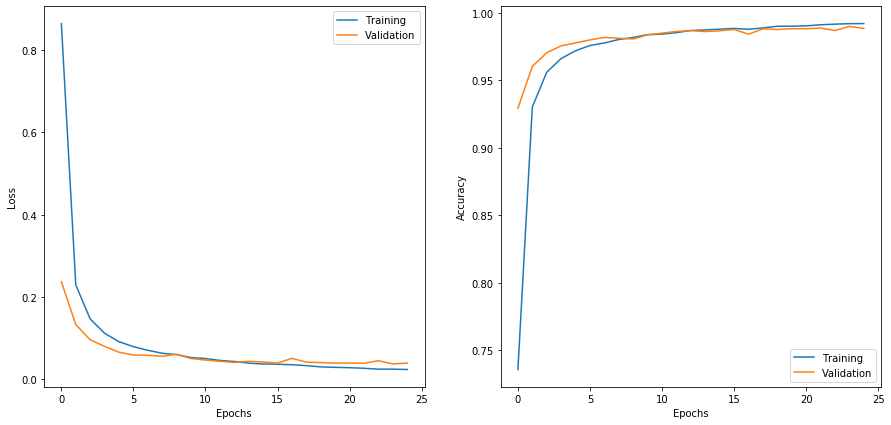
\includegraphics[width=\linewidth,height=4.5cm]{imgs/ValidationVsTrain.png}
	\caption{Train and Validation comparison}
	\label{fig:valVsTest}
\end{figure}
The model achieves an accuracy of $99.60\%$ in training and $98.85\%$ in validation.

\section*{Conclusions}
The performance of the test set obtains the result in Figure \ref{fig:test}.
\begin{figure}[!h]
	\centering
	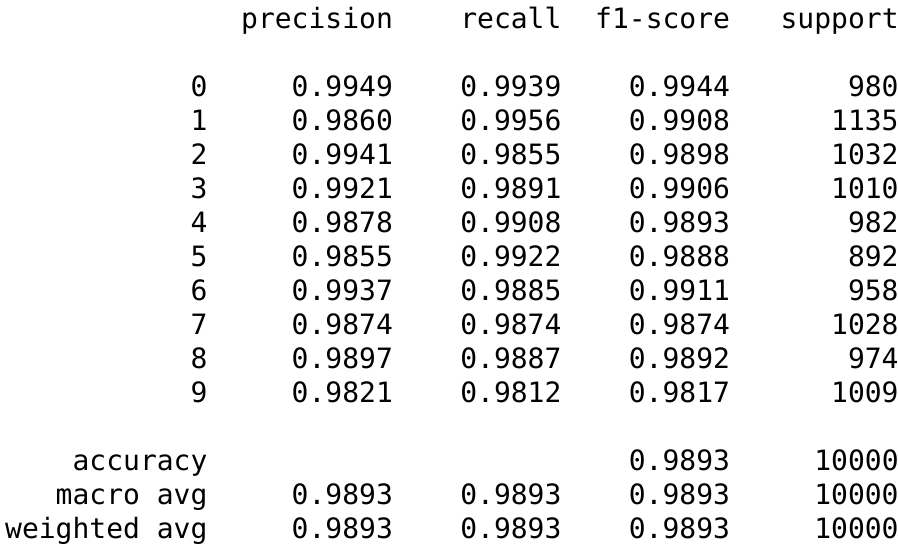
\includegraphics[width=10cm,height=4.5cm]{imgs/Test.png}
	\caption{Test Set classification report}
	\label{fig:test}
\end{figure}

The model achieves an accuracy of almost $98.93\%$, which is way better than the simple ANNs with a similar number of parameters. Moreover the Figure \ref{fig:valVsTest} indicates the model doesn't over or under-fits.

\end{document}
